In this chapter we wish to introduce different methods for modelling including hypothesis testing and cross-validation. In addition, methods for validation of the models will be introduced and applied on the constructed models.

\section{Modelling} \label{sec:modelling}
Based on the theory presented in chapter \ref{ch:Multip_linear_regresssion} we want to design a model and determine its coefficients. 
This will be done using the HOME dataset presented in chapter \ref{ch:introduction}. 
As argued there, the purpose is to predict prices based on selected independent variables that we suspect have an impact on the price of apartments in the selected cities.
The multiple regression model we will use in the following chapter is on the form:
\begin{align*}
    \textit{price} = \textit{cond} + \textit{size} + \textit{selling.period} + \textit{year.construct} + \textit{balcony} + \textit{renovation} + \textit{city} + year.sale
\end{align*}
To justify the inclusion of these variables, their $R$-squared value will be determined. 
This method is subjective but gives an impression of how important each independent variables is to explaining the variability in the dependent variable \textit{price}. 
The table below contains the $R$-squared and adjusted $R$-squared for models with each of the independent variables respectively.
\begin{table}[H]
\centering
\footnotesize
\begin{tabular}{lrrrrrrrr}
\toprule
\textbf{}          & \textit{cond} & \textit{size} & \textit{selling.period} & \textit{year.construct} & \textit{balcony} & \textit{renovation} & \textit{city} & \textit{year.sale} \\
\midrule
$R^2$ & 0.02027                & 0.5722              & 0.01356           & 0.1918                  & 0.02774        & 0.0002713              & 0.1262   & 0.2031     \\
$R^2_{Adj}$ & 0.02004                & 0.5722              & 0.01344           & 0.1897                  & 0.02762        & 0.0001537              & 0.1259  & 0.1956 \\
\bottomrule
\end{tabular}
\caption{\textit{R}-squared and adjusted \textit{R}-squared for the independent variables.}
\label{tab:r-squared}
\end{table}


Note that even if the $R$-squared is low, these parameters might still be significant and thereby improve the accuracy of the model, just not by much. 
The question is therefore rather if they are worth the added complexity.
We observe that with a tolerance level of 3 decimals, \textit{renovation} has coefficient of determination equal to zero and will therefore be excluded from the model.

Categorical variables like \textit{city} are potentially problematic, as these are accounted for by dummy variables, that add a different intercept for the model depending on which city is observed.
In order for this to give an accurate estimate of the cities influence on price, the estimated coefficients for the other variables need to be similar for models made from data of the different cities. 
To illustrate this we have plotted \textit{price} against \textit{size} in figure \ref{fig:Forskellig_haeldning}, for each of the cities.
\begin{figure}[H]
    \centering
    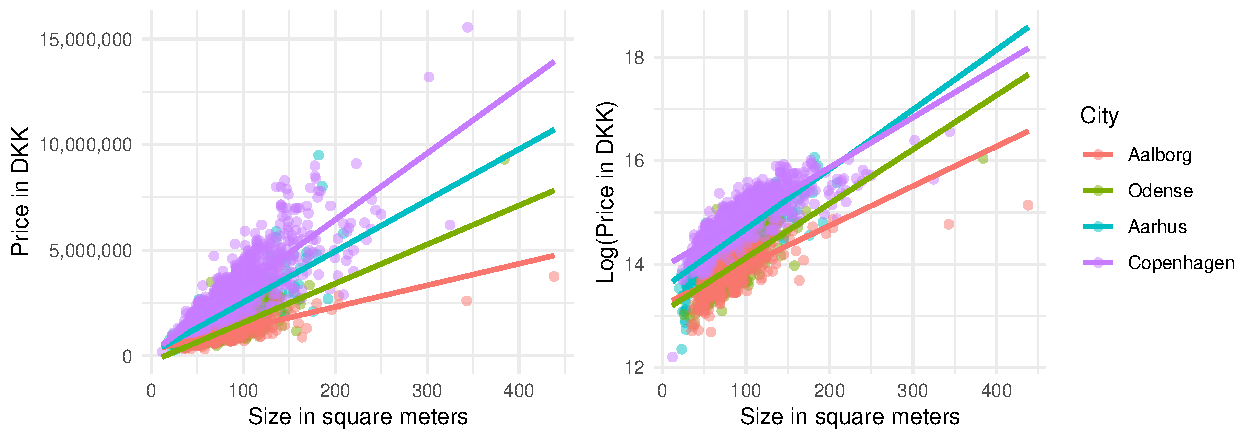
\includegraphics[width = 1\textwidth]{figures/Nanna/Forskellig_haeldning.pdf}
    \caption{The lines represents linear regressions where \textit{price} and $\log(price)$ is treated as the dependent variable and size in square meters the dependent variable.}
    \label{fig:Forskellig_haeldning}
\end{figure}
Making linear models for each of these groups, we find that the difference in slope between the models is significant.
For now this is simply seen from the figure \ref{fig:Forskellig_haeldning} and the coefficients in table \ref{tab:my-table}, but this will be explored in more detail in chapter \ref{ch:hypothesis_testing}. 


\begin{table}[H]
\centering
\begin{tabular}{lrrrrrrr}
\toprule
\textbf{By}                                                                                       & \textbf{term}                & 
\textbf{estimate}            & \textbf{std.error}           & \textbf{statistic}           & \textbf{p.value}             \\
\midrule
Aarhus                                                                                & (Intercept)                  & 13.5                      & 0.0257                       & 527                         & 0                      \\
Aarhus                                                                            &  \textit{size}                   & 0.0115                       & 0.000325                         & 35.5                         & 1.24e-163                    \\
\addlinespace
Odense                                                                            &  (Intercept)                  & 13.1                     & 0.0310                       & 421                        & 0                    \\
Odense                                                                             &  \textit{size}                   & 0.0105                       & 0.000379                         & 27.7                        & 3.99e-105                    \\
\addlinespace
Aalborg                                                                           &  (Intercept)                  & 13.2                      & 0.0378                       & 350                         & 0                     \\
Aalborg                                                                            &  \textit{size}                   & 0.00766                       & 0.000425                         & 18.0                         & 1.14e- 53                    \\
\addlinespace
Copenhagen                                                                     &  (Intercept)                  & 13.9                      & 0.0196                       & 709.                        & 0                      \\
Copenhagen                                                                       &  \textit{size}                   &  0.00968                       & 0.000206                         & 47.1                        & 5.23e-273 \\                          
\bottomrule
\end{tabular}
\caption{Summary for the linear models $\log(price) \sim size$ in figure \ref{fig:Forskellig_haeldning}.}
\label{tab:my-table}
\end{table}

Adding \textit{size} as a parameter therefore decreases accuracy, and it might be wise to make separate models for each city. 
Note that this example only considers the size, and not the other categorical variables; \textit{cond} and \textit{year.construction}.

Below in figure \ref{fig:Opfoerelsesaar_plot} is a plot of how the parameter \textit{year.construct} influences the price of apartments.
As reflected by the $R$-squared value seen in table \ref{tab:r-squared}, the price varies significantly depending on the year of construction. 
We thereby conclude that this parameter is important and should be included in the model. 

\begin{figure}[H]
    \centering
    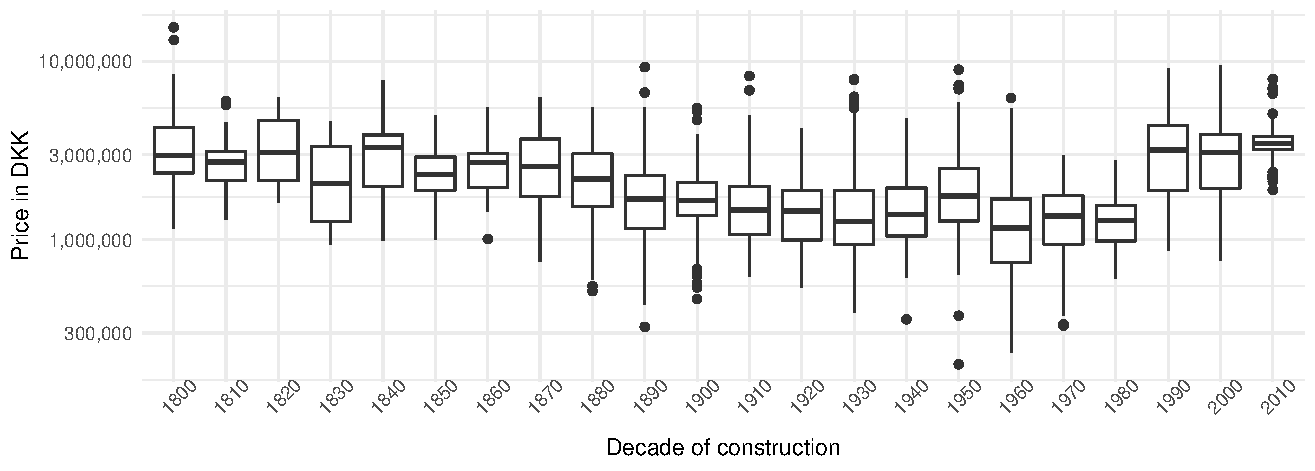
\includegraphics[width = 1\textwidth]{figures/Nanna/Opfoerelsesaarplot.pdf}
    \caption{}
    \label{fig:Opfoerelsesaar_plot}
\end{figure}

From the left side of figure \ref{fig:Forskellig_haeldning} we see that the observations are heteroskedastic and their variance increases as "Boligareal" increases. 
In order to satisfy the Gauss-Markov assumptions the observations need to have constant variance and we therefore need to transform the data, to remedy this. 
The logarithm is a variance stabilizing function, so using this on both "Kontantpris" and "Boligareal" we see that the residuals seem to be approximately normally distributed around the regression line, as illustrated in figure \ref{fig:Log_Model_plot}. 

\begin{figure}[H] 
    \centering
    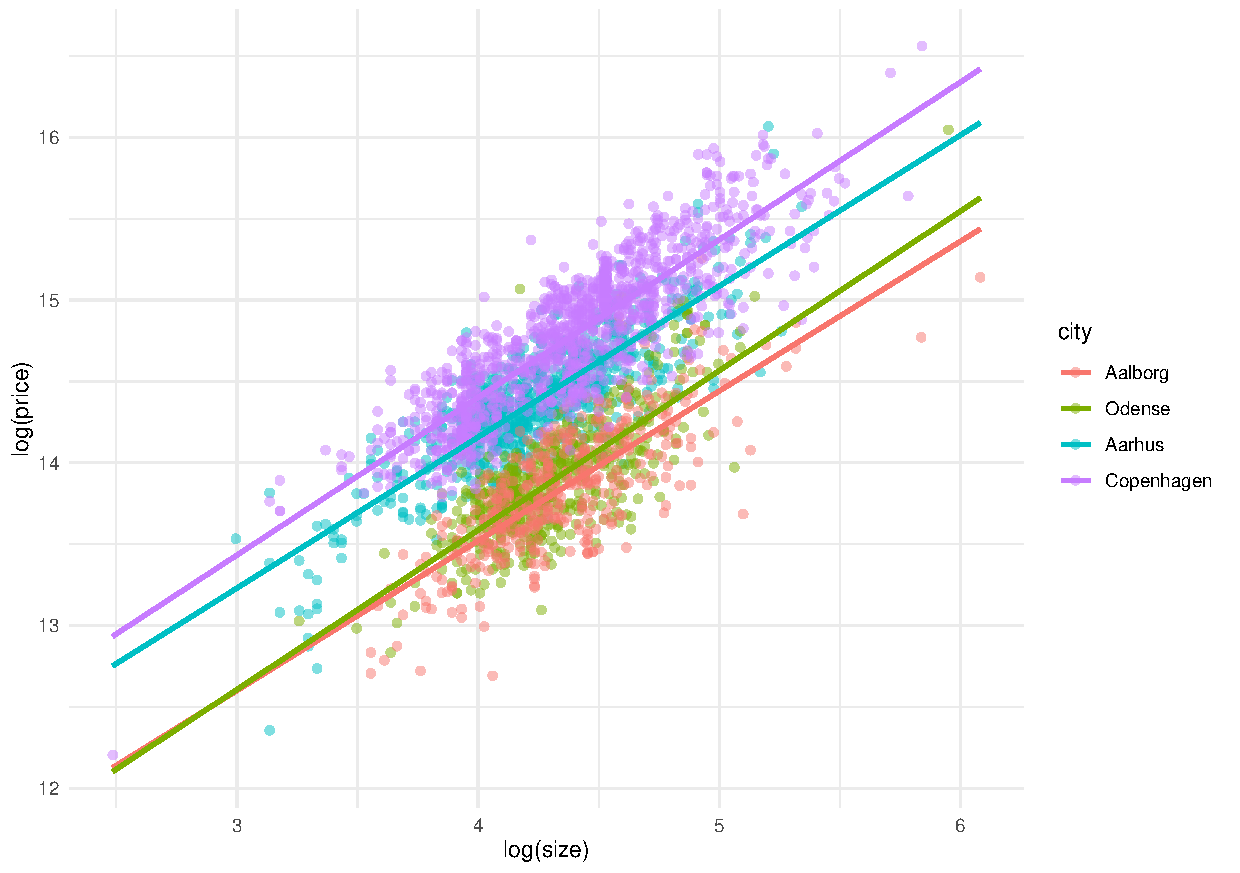
\includegraphics[width = 0.6\textwidth]{figures/Nanna/Plot_forskellig_haeldning.pdf}
    \caption{Plot of log(Kontantpris) = $\beta_0 + \beta_1 log(Boligareal)$ }
    \label{fig:Log_Model_plot}
\end{figure}

In the same manner we conclude, that the variance of the price is more homoskedastic after the log transformation, for all the independent variables listed in the model.
As with 'Boligareal', taking the logarithm also improves the coefficient of determination for 'Liggetid'. 
Therefore we will continue to work with the following model
%These variables will be investigated more effectively in the next chapter, and so this is the model we will continue to work with
\begin{lstlisting}
    log(Kontantpris) ~ Boligtilstand + log(Boligareal) + Liggetid
    + Opfoerelsesaar + Altan.
\end{lstlisting}